%-------------------------------------------------------------------------------
% 请勿删除本注释
% Free Response Question 3
%
% 指引:
% 如在小问之前有通用问题描述,请放置于此
%-------------------------------------------------------------------------------
\begin{figure}[H]
\centering
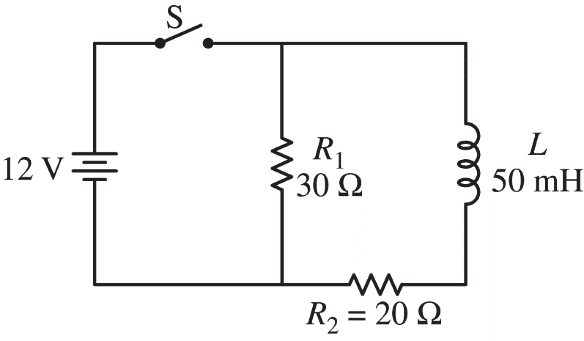
\includegraphics[scale=0.3]{images/img-025-039.png}
\end{figure}


\question
The circuit shown above is constructed using an ideal $12 \mathrm{~V}$ battery, an ideal switch $\mathrm{S}$, and two resistors and an inductor with the values shown. Switch $S$ is closed. After a long time, the circuit reaches steady-state conditions. % 请删除并替换本行,与上一行 \question 之间不要留空行

\begin{parts}

%-------------------------------------------------------------------------------
% 请勿删除本注释
% Part (a)
%
% 指引:
% 如在小问之前有通用问题描述,请放置于此
%-------------------------------------------------------------------------------

\part
Calculate the current through $R_{1}$. % 请删除并替换本行,与上一行 \part 之间不要留空行

%-------------------------------------------------------------------------------
% 请勿删除本注释
% Part (b)
%
% 指引:
% 如在小问之前有通用问题描述,请放置于此
%-------------------------------------------------------------------------------

\part
Calculate the current through the battery. % 请删除并替换本行,与上一行 \part 之间不要留空行

%-------------------------------------------------------------------------------
% 请勿删除本注释
% Part (c)
%
% 指引:
% 如在小问之前有通用问题描述,请放置于此
%-------------------------------------------------------------------------------
The switch is then opened at time $t=0$.

\part
Determine the current in the inductor immediately after the switch is opened. % 请删除并替换本行,与上一行 \part 之间不要留空行

%-------------------------------------------------------------------------------
% 请勿删除本注释
% Part (d)
%
% 指引:
% 如在小问之前有通用问题描述,请放置于此
%-------------------------------------------------------------------------------

\part
 % 请删除并替换本行,与上一行 \part 之间不要留空行
\begin{subparts}
\subpart Determine the current in resistor $R_{1}$ immediately after the switch is opened.
\subpart Which of the following statements is correct about the current through $R_{1}$ immediately after the switch is opened?

\underline{\qquad}The current is up through $R_{1}$. \qquad   \underline{\qquad}The current is down through $R_{1}$.

\underline{\qquad}There is no current through $R_{1}$.

Justify your answer.

\end{subparts}

%-------------------------------------------------------------------------------
% 请勿删除本注释
% Part (e)
%
% 指引:
% 如在小问之前有通用问题描述,请放置于此
%-------------------------------------------------------------------------------

\part
Immediately after the switch is opened, is the top end or bottom end of the inductor at the higher electric potential?

\underline{\qquad}Top end  \qquad \underline{\qquad}Bottom end

Justify your answer. % 请删除并替换本行,与上一行 \part 之间不要留空行

%-------------------------------------------------------------------------------
% 请勿删除本注释
% Part (f)
%
% 指引:
% 如在小问之前有通用问题描述,请放置于此
%-------------------------------------------------------------------------------

\part
On the axes below, sketch a graph of the potential difference $V$ across the inductor as a function of time after the switch is opened. Explicitly label the vertical axis intercept with a numerical value. % 请删除并替换本行,与上一行 \part 之间不要留空行

\begin{figure}[H]
\centering
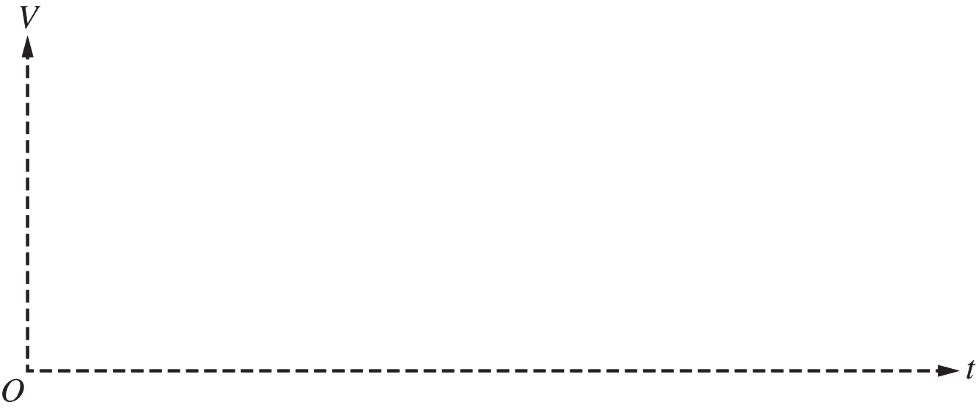
\includegraphics[scale=0.3]{images/img-027-040.png}
\end{figure}

%-------------------------------------------------------------------------------
% 请勿删除本注释
% Part (g)
%
% 指引:
% 如在小问之前有通用问题描述,请放置于此
%-------------------------------------------------------------------------------

\part
Write but DO NOT solve a differential equation that could be solved for the current through the inductor as a function of time after the switch is opened. % 请删除并替换本行,与上一行 \part 之间不要留空行

\end{parts}


